\documentclass{article}
\usepackage[T1]{fontenc}
\usepackage[utf8]{inputenc}
\usepackage{graphicx}
\usepackage{float}
\usepackage[polish]{babel}
\usepackage{amsmath}
\usepackage[a4paper, margin=1in]{geometry}

\title{Metody numeryczne - laboratorium 2}
\author{Natan Tułodziecki}
\date{10 marca 2025}

\begin{document}

\maketitle

\section{Analiza błędu przybliżenia pochodnej}

\begin{figure}[H]
    \centering
    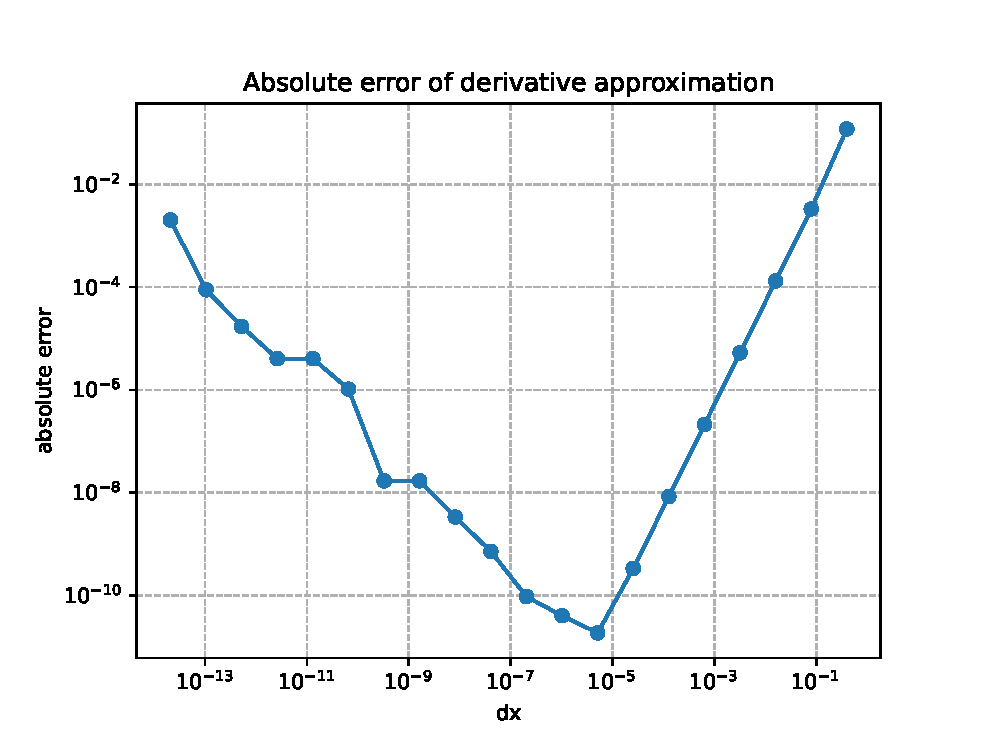
\includegraphics[width=1\linewidth]{Figure_1.eps}
    \caption{Wartość bezwzględna błędu przybliżenia pochodnej}
    \label{fig:blad}
\end{figure}

Wykres błędu w skali log-log (rys. \ref{fig:blad}) wykazuje charakterystyczny kształt litery „U”, co jest efektem działania dwóch głównych źródeł błędów:

\begin{itemize}
    \item \textbf{Błąd obcięcia} – dla dużych wartości \( dx \) metoda centralnej różnicy przybliża pochodną z dokładnością rzędu \( O(dx^2) \), co prowadzi do większego błędu obliczeń.
    \item \textbf{Błąd zaokrągleń} – dla bardzo małych wartości \( dx \), różnice funkcji stają się porównywalne z precyzją maszynową, co skutkuje niestabilnością numeryczną i wzrostem błędu.
\end{itemize}

Wartość \( dx \), dla której błąd osiąga minimum, to optymalny krok różnicowy, pozwalający na najbardziej precyzyjne przybliżenie pochodnej. Wartość ta została wyznaczona jako:

\[
dx \approx {best\_dx}
\]

\section{Analiza przybliżenia pochodnej}

\begin{figure}[H]
    \centering
    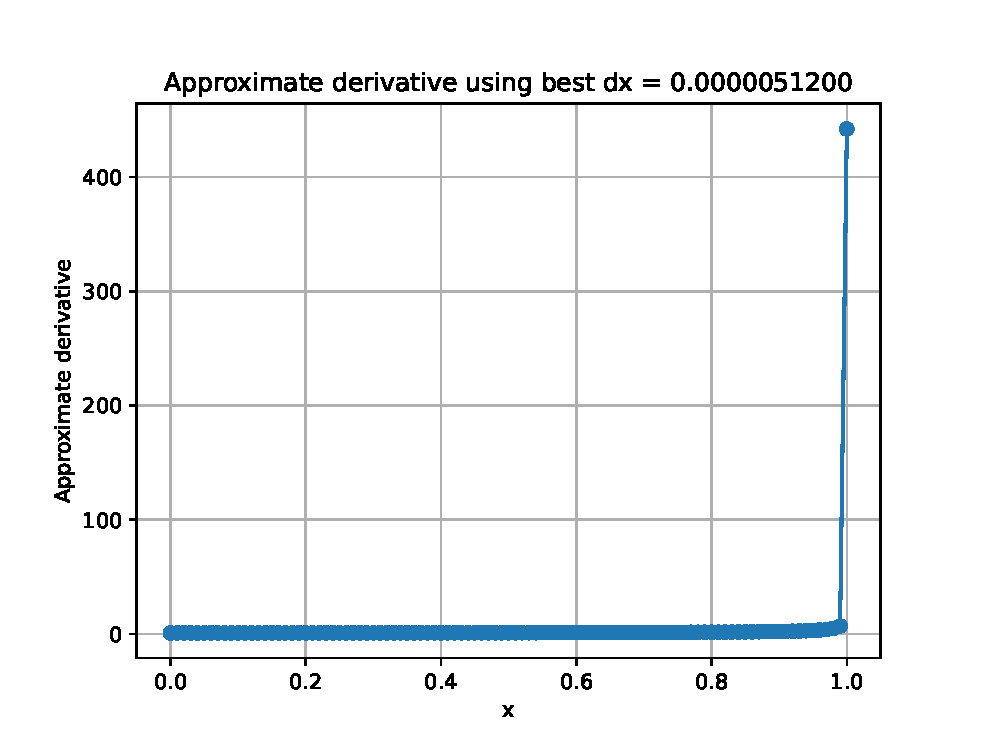
\includegraphics[width=1\linewidth]{Figure_2.eps}
    \caption{Przybliżenie pochodnej dla \( dx \) minimalizującego błąd}
    \label{fig:pochodna}
\end{figure}

Wykres na rysunku \ref{fig:pochodna} przedstawia wartości przybliżonej pochodnej funkcji \( \arcsin(x) \) wyznaczonej metodą centralnej różnicy dla optymalnej wartości \( dx \). Można zauważyć kilka kluczowych zależności:

\begin{itemize}
    \item W zakresie \( x \in [0, 0.9] \) aproksymacja pochodnej jest bardzo dokładna i zgodna z analitycznym wzorem \( \frac{1}{\sqrt{1 - x^2}} \).
    \item W miarę zbliżania się \( x \) do 1, wartości pochodnej gwałtownie rosną. Jest to zgodne z zachowaniem rzeczywistej pochodnej funkcji \( \arcsin(x) \), która dąży do nieskończoności, gdy \( x \to 1 \).
    \item Dla wartości \( x \) bardzo bliskich 1 (np. \( x > 0.98 \)), obliczona pochodna staje się niestabilna numerycznie, co objawia się gwałtownym wzrostem wartości. Efekt ten wynika z ograniczonej precyzji numerycznej oraz faktu, że mianownik wyrażenia \( \frac{1}{\sqrt{1 - x^2}} \) zbliża się do zera, powodując znaczne powiększenie błędów obliczeniowych.
\end{itemize}

Podsumowując, wykres ilustruje wysoką dokładność aproksymacji w szerokim zakresie \( x \), jednak w pobliżu \( x \to 1 \) precyzja maleje ze względu na naturę funkcji oraz ograniczenia numeryczne.

\end{document}
